\documentclass[11pt]{article}

\usepackage{bookmark}
\usepackage{float}
\usepackage{booktabs}
\usepackage{graphicx}
\usepackage{csvsimple}
\usepackage{tabularx}


% DOCUMENT SETTINGS
\setlength{\parskip}{0.5em}
\setlength{\parindent}{0pt}
\graphicspath{{../outputs/}}

\newcommand{\datapath}{../outputs/}

% TITLE
\title{Model Comparison for Financial Sentiment Analysis}
\author{Riccardo Scala}
\date{\today}


\begin{document}

    \maketitle
    \medskip
    \section{Introduction}

    Financial sentiment analysis is a Natural Language Processing (NLP) task aimed at automatically identifying the sentiment expressed in financial texts such as news articles, market reports and investor communications.

    The task is particularly relevant in finance because market sentiment may influence investment decisions, risk perception and stock price movements. However, financial language presents several challenges, including implicit sentiment, ambiguity, domain-specific terminology, and highly contextual expressions.

    The objective of this project is to compare two different approaches for financial sentiment classification:

    \begin{itemize}
        \item a classical NLP baseline based on TF-IDF + Logistic Regression;
        \item a dense sentence embedding-based model + Logistic Regression.
    \end{itemize}

    The models are evaluated and compared using classification metrics, confusion matrices, and qualitative error analysis.

    The analysis was carried out in Python using \textit{scikit-learn} for TF-IDF vectorization, Logistic Regression classification and evaluation metrics, and \textit{sentence\_transformers} for embedding-based text representations.


    \section{Dataset}

    The dataset used for this analysis was downloaded from \textit{Kaggle} and is based on a combination of the \textit{FiQA} and \textit{Financial PhraseBank} datasets.

    Initially, the dataset contained 5842 financial sentences labelled according to their sentiment: \textbf{negative, neutral, positive}

    Following an initial data inspection, duplicate sentences were found and removed, bringing the size of the dataset down to 5322 items. Class imbalance was detected as well: as displayed in figure 1, neutral-labled sentences constitute roughly the 54\% of the entire corpus, while the least represented class, the negative, represents only 11\%.

    After this first check, only minimal preprocessing was applied: sentences were converted to string objects and leading/trailing whitespaces were removed.

    More aggressive preprocessing techniques such as stemming, lemmatization, stopword removal, or number removal were intentionally avoided in order to preserve potentially relevant financial information. In fact, in financial sentiment analysis, numbers, negations, and domain-specific terminology may carry important semantic signals that could be lost through excessive text normalisation.

    The dataset was divided into train and test sets using an 80/20 split with stratification to preserve class proportions.

    \medskip
    \begin{figure}[htbp]
        \centering
        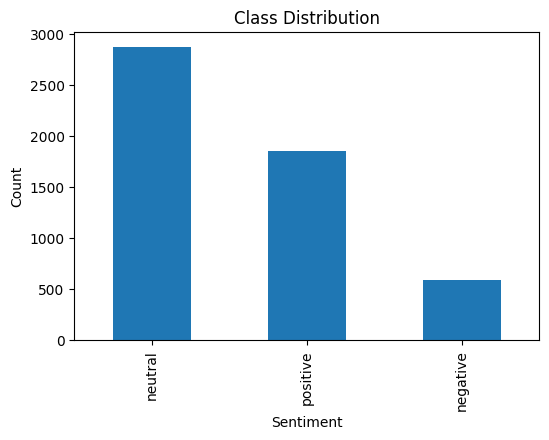
\includegraphics[width = 0.55\textwidth]{class_distribution.png}
        \caption{Dataset class distribution}
    \end{figure}


    \section{Methods}

    \subsection{TF-IDF Baseline}

    The first approach is based on TF-IDF vectorization combined with Logistic Regression.

    TF-IDF produces a sparse bag-of-words representation where each sentence is converted into a vector of weighted lexical features. The weighting scheme combines:

    \begin{itemize}
        \item \textbf{Term Frequency (TF)}, representing the relative frequency of a word in a sentence:
        
        \[
        tf(t,d) = \frac{\#(t\ in\ d)}{total\ number\ of\ tokens\ in\ d}
        \]

        \item Inverse Document Frequency (IDF), which rewards terms that are rare across the corpus.
        
        \[
        idf(t,D) = \log \left( \frac{N}{|\{ d \in D : t \in d \}|} \right)
        \]

        where:
        \begin{itemize}
            \item \(N\) is the total number of documents in the corpus;
            \item \(|\{ d \in D : t \in d \}|\) is the number of documents containing term \(t\).
        \end{itemize}

    \end{itemize}

    The resulting measure \( tfidf(t,d,D) = tf(t,d) \cdot idf(t,D) \) rewards words that are frequent in a given sentence but not too frequent in the corpus as a whole.
    
    The TF-IDF representation was built using both unigrams and bigrams, allowing the model to capture both individual word importance and short contextual expressions.

    The classifier used is multinomial Logistic Regression with balanced class weights to compensate for dataset imbalance. The model predicts sentiment classes using TF-IDF representations of the input text.


    \subsection{Embedding-based model}

    The second approach replaces sparse lexical vectors with dense semantic sentence embeddings.

    Unlike TF-IDF representations, which are based on term frequencies and treat words as largely independent features, embedding-based representations encode sentences into dense continuous vectors capable of capturing semantic and contextual relationships between words. In this vector space, sentences with similar meanings are mapped to nearby representations even when they do not share the same vocabulary.

    The sentence embeddings used in this work are generated using the all-MiniLM-L6-v2 transformer model, which encodes each sentence into a 384-dimensional vector representation. Transformer-based models leverage self-attention mechanisms to capture contextual dependencies between words, allowing the representation of a term to vary depending on the surrounding context.

    The resulting embeddings are then used as input features for a Logistic Regression classifier, similarly to the TF-IDF approach.


    \subsection{Evaluation Metrics}

    The models are evaluated using the following metrics:
    \begin{itemize}
        \item \textbf{Accuracy}: measures the proportion of correctly classified sentences over the total number of observations;
        \item \textbf{Precision}: measures how many sentences predicted as belonging to a class are actually correct;
        \item \textbf{Recall}: measures how many true examples of a class are correctly identified by the model;
        \item \textbf{Macro F1-score}: combines precision and recall into a single metric, rewarding models that perform well on both measures. The \textbf{Macro F1-score} is computed as the average F1-score across all classes, assigning the same importance to each of them.
    \end{itemize}

    Macro F1-score is particularly important due to dataset imbalance, since it assigns equal importance to all classes independently of their frequency.


    \section{Results}

    As shown in Table~1 the embedding-based approach achieves better overall performance, particularly on the minority negative class, where semantic representations appear more effective at capturing contextual meaning and implicit sentiment. The TF-IDF model, however, remains competitive and achieves slightly stronger results on some neutral examples.

    \begin{table}[htbp]
        \centering
        {\footnotesize
        \csvautotabular{\detokenize{../outputs/metrics_summary_transposed.csv}}
        }
        \caption{Summary of model metrics}
        \label{tab:metrics_summary}
    \end{table}

    The confusion matrices further highlight the different behaviour of the two approaches. The embedding-based model achieves substantially higher recall on the negative class, while TF-IDF performs slightly better on some neutral examples.

    \begin{figure}[h]
        \centering
        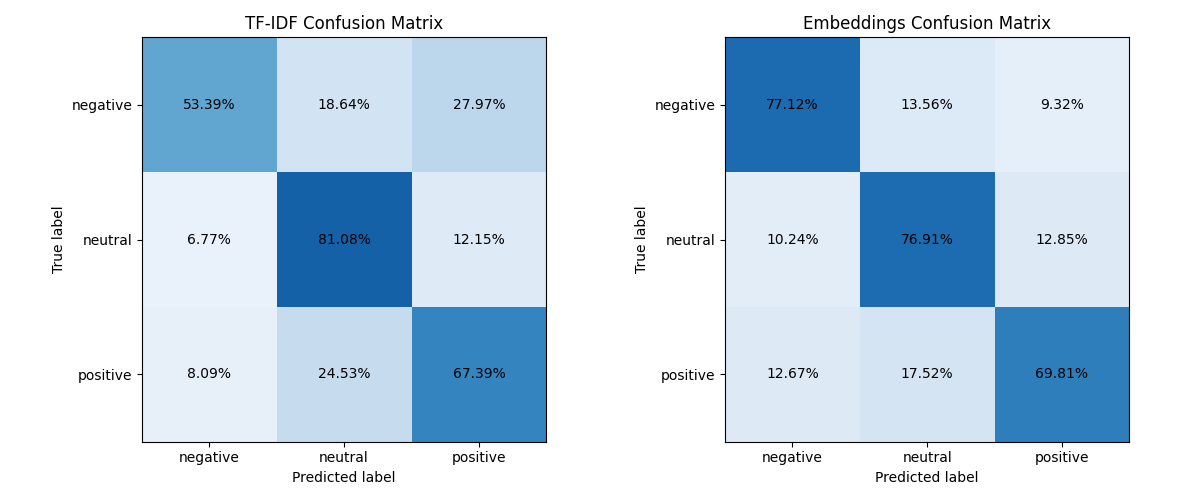
\includegraphics[width = 0.99\textwidth]{confusion_matrices_comparison.png}
        \caption{Confusion matrices for the TF-IDF and embedding-based models}
    \end{figure}


    \section{Error Analysis}

    A sample of misclassified examples is analyzed in order to identify systematic weaknesses of both approaches.

    TF-IDF errors are often caused by implicit sentiment, sarcasm, contextual ambiguity or forward-looking financial language.

    In contrast, embedding-based errors are more frequent in short financial statements or highly technical sentences where sentiment is weak or only indirectly expressed.

    \medskip
    \begin{table}[h]
        \centering
        \footnotesize

        \begin{tabularx}{\textwidth}{lXccc}
            \toprule
            ID & Sentence & True & TF-IDF & Emb \\
            \midrule
            5645 & \$SPY Tomorrow party time for the Bears!! \$GOOG and \$MSFT -5.5\% & negative & positive & negative \\
            4878 & EUR 152.4 mn of this was net interest income & neutral & positive & neutral \\
            5590 & Britain's FTSE steadies, supported by Dixons Carphone & positive & positive & neutral \\
            244 & We went to the market with yield guidance of the 7.25 \% area, which gave us the flexibility to go up or down by 1-8th & neutral & neutral & positive \\
            1095 & \$SINA even though the "report" is untrue and has been proven unture, the damage is done. No one wants to touch it now & negative & neutral & negative \\
            823 & The new technology improves the glass quality and consistency while increasing throughput & positive & neutral & positive \\
            3718 & As a result, the Russia's import restrictions on Finnish dairy companies will be canceled on 6 August 2010 & positive & neutral & negative \\
            4324 & Oriola-KD expects its invoicing in 2008 to be higher than the comparable invoicing of 2007 & positive & neutral & positive \\
            1137 & After the takeover, Cramo will become the second largest rental services provider in the Latvian market & positive & positive & neutral \\
            441 & \$ISRG - ISRG Short - http://stks.co/f1vVU http://stks.co/c1qrm & negative & negative & neutral \\
            \bottomrule
        \end{tabularx}

        \tiny\caption{Error sample}
    \end{table}

    Most misclassifications can be explained by the known limitations of the two models. For example, in sentence 5645, the TF-IDF fails to capture the sarcasm through which the bad news is conveyed. On the other hand, in sentence 441, the embedding-based model struggles to get the context in such short sentence, while TF-IDF recognise "Short" alone as negative.


    \section{Conclusion}

    Both models achieve satisfactory performance on the financial sentiment classification task, although they exhibit different strengths and weaknesses.

    The TF-IDF model performs generally well and remains highly interpretable, but due to its architecture it struggles with contextual meaning, implicit sentiment, and financial ambiguity. This may be the main reason why the model struggles more often with the negative class: negative financial news is often expressed in a less direct way than other sentiments, sometimes through subtle wording, sarcasm or metaphors.

    In contrast, the embedding-based approach demonstrates better generalisation capabilities and improved performance on the minority negative class, suggesting that semantic representations are more effective at capturing subtle financial language. Still, it is important to note the higher computational cost required by this model compared with TF-IDF, whose efficiency remains one of its main advantages.

    In conclusion, although embedding-based model achieves overall better performance, model selection should also take into account other factors, such as dataset structure, computational constraints and whether the expected performance improvement justifies the additional resource demand.

\end{document}
